\documentclass[12pt,a4paper, openany]{memoir}

% Required packages
\usepackage[utf8]{inputenc}
\usepackage[T1]{fontenc}
\usepackage{lmodern}
\usepackage{amsmath}
% Math symbols (\mathbb, \mathcal, etc.)
\usepackage{amssymb}
% Improve micro-typography to reduce overfull boxes
\usepackage[final]{microtype}
% Use Polish as main language; provide=* avoids error when language ini is present but ldf missing
\usepackage[main=polish,provide=*]{babel}
\usepackage{graphicx}
\usepackage{geometry}
\usepackage{wrapfig}
\usepackage{listings}
\usepackage{xcolor}
\usepackage{hyperref}
\usepackage{xurl}
\hypersetup{hidelinks, hypertexnames=false}
\usepackage{pgfplots}
\pgfplotsset{compat=1.18}
\usepackage{float}
% Allow more floats and flexible page layout (helps with Underfull \vbox)
\renewcommand{\topfraction}{0.95}
\renewcommand{\floatpagefraction}{0.9}
\renewcommand{\textfraction}{0.05}
\renewcommand{\bottomfraction}{0.9}
\setcounter{topnumber}{5}
\setcounter{bottomnumber}{5}
\setcounter{totalnumber}{10}

\definecolor{codegreen}{rgb}{0,0.6,0}
\definecolor{codegray}{rgb}{0.5,0.5,0.5}
\definecolor{codepurple}{rgb}{0.58,0,0.82}
\definecolor{backcolour}{rgb}{0.95,0.95,0.92}

% \chapterstyle{veelo}

\lstdefinestyle{codeListingStyle}{
    backgroundcolor=\color{backcolour},   
    commentstyle=\color{codegreen},
    keywordstyle=\color{magenta},
    numberstyle=\tiny\color{codegray},
    stringstyle=\color{codepurple},
    basicstyle=\ttfamily\footnotesize,
    breakatwhitespace=false,         
    breaklines=true,                 
    captionpos=b,                    
    keepspaces=true,                 
    numbers=left,                    
    numbersep=5pt,                  
    showspaces=false,                
    showstringspaces=false,
    showtabs=false,                  
    tabsize=2
}
\usepackage{graphics}

\usepackage{titlesec}
\titleformat{\chapter}[display]
  {\normalfont\Large\raggedleft}
  {\MakeUppercase{\chaptertitlename}%
    \rlap{ \resizebox{!}{1.5cm}{\thechapter} \rule{7cm}{1.5cm}}}
  {10pt}{\Huge}
\titlespacing*{\chapter}{0pt}{5pt}{20pt}

\setcounter{secnumdepth}{3}
\setcounter{tocdepth}{3}
% Set page margins
\geometry{top=0cm, bottom=2cm, left=2cm, right=2cm}

\begin{document}

% Enable page numbers on all pages
\pagestyle{plain}
\pagenumbering{arabic}
% Ensure chapter-opening pages also use the same pagestyle
\aliaspagestyle{chapter}{plain}
% Suppress page number on the very first page only
\thispagestyle{empty}

% Avoid stretching pages to equal height; reduces Underfull \vbox warnings
\raggedbottom

% Gently reduce Overfull \hbox warnings by allowing tiny extra stretch in lines
\emergencystretch=1em

% Add image at the top of the page
\begin{figure}[t!]
    \centering
    \includegraphics[width=1\textwidth]{images/PJATK_PL_poziom_1.png}
    \label{fig:top-image}
\end{figure}

% Centered content
\begin{center}
\vspace{2cm}

{\Large \textbf{Wydział Informatyki}}

\vspace{1.5cm}

{\large  \textbf{Systemy Inteligentne i Data Science}}

\vspace{0.5cm}

Inteligentne Systemy Przetwarzania Danych

\vspace{2cm}

{\large  \textbf{Michał Lichtarski}} \\
Nr albumu s27643

\vspace{0.5cm}

{\large  \textbf{Marcin Ziółkowski}} \\
Nr albumu s27597

\vspace{2cm}

{\Large \textbf{Tytuł pracy dyplomowej}}

\end{center}

\vfill

\begin{flushleft}
\hspace*{0.5\textwidth}Praca inżynierska \\
\hspace*{0.5\textwidth}Promotor Adam Szmigielski
\end{flushleft}


\vspace{2.5cm}

\begin{center}
Warszawa, luty 2026
\end{center}


\newgeometry{top=2cm, bottom=2cm, left=2.5cm, right=2.5cm}

\tableofcontents

\section*{Streszczenie}

Celem niniejszej pracy jest przedstawienie działania oraz implementacji równoległego silnika szachowego opartego na algorytmie przeszukiwania drzewa Monte Carlo wspomaganego siecią neuronową. Zostanie przedstawiony proces przetwarzania danych szachowych wraz z niezbędną modyfikacją biblioteki szachowej.
W pracy zostaną omówione ulepszenia zarówno sieci neuronowej jak i samego MCTS, które zostały wprowadzane na przestrzeni ostatnich kilku lat. Na końcu zostaną przedstawione wyniki ewaluacji samej sieci neuronowej oraz porównanie opisywanego silnika z silnikiem Stockfish.

\textbf{Słowa kluczowe} – monte carlo tree search, sieć neuronowa, szachy, wieloprocesowość

\section*{Wstęp}

Żyjemy w dynamicznie rozwijającym się technologicznie świecie, w którym algorytmy uczenia maszynowego odgrywają coraz to większą rolę w różnych dziedzinach życia. Możemy je spotkać nawet w szachach. Prawie każdy z nas zna strony internetowe gdzie można rywalizować z różnymi graczami, czy nawet z modelami. Dla zobrazowania jak algorytmy szachowe są skomplikowanym zadaniem Claude Shannon w swoim artykule z 1950 roku \textit{Programming a Computer for Playing Chess} oszacował, że liczba wszystkich różnych kombinacji partii w szachach wynosi około $10^{120}$, co jest nazwane dzisiaj liczbą Shannon'a. Również opisał jak powinien wyglądać algorytm heurystyczny, który bierze pod uwagę najbardziej obiecujące ruchy "Select the variations to be explored by some process so that the machine does not waste its time in totally pointless variations.". Gdyż jak sam podkreślił, metodą brute force jest to nieosiągalne. Dało to początek rozwoju algorytmów takich jak minimax, czy monte Carlo tree search, które są obecnie szeroko stosowane do dzisiaj.

Jak bardzo zmieniły się algorytmy szachowe na przestrzeni lat dobrze obrazuje książka Huberta Dreyfusa \textit{Alchemy and Artificial Intelligence} z 1965 roku, w której autor napisał że nie ma obecnie algorytmu szachowego, który byłby wstanie grać na amatorskim poziomie "Still no chess program can play even amateur chess". Gdzie zaledwie 20 lat później, w 1988 roku, program szachowy \textit{Deep Thought} wygrał z arcymistrzem szachowym Bentem Larsenem. W 1997 roku komputer \textit{Deep Blue} pokonał Kasparowa w meczu z standardową kontrolą czasu, a w 2017 roku program AlphaZero opracowany przez Google pokonał algorytmy szachowe, takie jak Stockfish i Elmo.
\section*{Środowisko}
Przedstawione rozwiązanie zostało zaimplementowane w języku Python. Podyktowane to było przede wszystkim dużą ilością dostępnych wysokopoziomowych bibliotek, które znacznie przyśpieszają opracowanie i testowanie algorytmów.

Ze względu na bardzo duży koszt obliczeniowy trenowania sieci, został wykorzystany serwer z procesorem Intel Xeon E5-2686v4 wraz z 128GB pamięci RAM oraz kartami graficznymi Nvidia RTX 3080 12gb oraz NVIDIA Tesla v100 16gb. Jako system operacyjny został użyty PROXMOX na którym zostały uruchomione odpowiednie maszyny wirtualne z systemem Ubuntu desktop z bezpośrednim dostępem do GPU. Takie rozwiązanie pozwala na dużą elastyczność ze względu na łatwy dostęp do zasobów serwera poprzez przeglądarkę internetową z dowolnego miejsca. Ponadto umożliwia nieprzerwane trenowanie modeli.

\section*{Wykorzystane biblioteki}
Język Python, który jest interpretowanym językiem wysokiego poziomu, wymaga używania bibliotek napisanych w językach niższego poziomu, w celu zapewnienia akceptowalnej wydajności.
W celu implementacji przedstawionego rozwiązania zostały wykorzystane następujące biblioteki:

\begin{itemize}
	\item \textbf{NumPy}: służy do obliczeń naukowych; umożliwia bardzo szybkie operacje na macierzach i wektorach.
	\item \textbf{Matplotlib}: umożliwia tworzenie wykresów i wizualizację danych.
	\item \textbf{PyTorch}: biblioteka do implementacji sieci neuronowych; umożliwia elastyczne tworzenie architektur sieci oraz łatwe wykorzystanie GPU, co znacząco przyspiesza trenowanie modeli.
\end{itemize}

\setcounter{chapter}{0}

\chapter{Tworzenie zbioru danych}
Tworzenie zbioru danych jest bardzo istotnym etapem w uczeniu maszynowym. Od ich jakości oraz formatu zależy skuteczność modelu. Dane użyte do trenowania zostały pobrane ze strony \textit{lichess.org}. Został wykorzystany zbiór \textit{Lichess Elite Database} zawierający rozgrywki graczy na poziomie większym niż 2300, co jest bardzo wysokim wynikiem. Co ważne, zbiór ten nie zawiera powtórzeń, a także rozgrywek czasowych dzięki temu model nie uczy się złych, nietypowych strategii tworzonych pod presją czasu. Pobrany zbiór danych składa się z kilku plików o rozszerzeniu \textit{.pgn}, z których każdy zawiera około miliona partii szachowych

\section{Format danych PGN}
Format PGN jest powszechnie stosowanym sposobem przechowywania partii szachowych. W danym pliku może znajdować się dowolna ilość gier. Każda z nich ma między innymi nazwy graczy, wynik oraz stos ruchów. Taki sposób zapisu jest bardzo efektywny pamięciowo, gdyż nie zapisuje on pozycji na planszy w każdej turze, a jedynie wykonywane ruchy. Dodatkowym atutem jest gotowa biblioteka python-chess do dekodowania pliku oraz rozgrywania partii.

\vspace{0.5cm}

\begin{lstlisting}[
    language=Python, 
    caption=przykład pliku PGN,
    inputencoding=utf8,
    basicstyle=\ttfamily\footnotesize,
    xleftmargin=0.1cm,
    showspaces=false,
    showstringspaces=false,
    showtabs=false,
    keepspaces=true
]
[Event "F/S Return Match"] 
[Site "Belgrade, Serbia JUG"] 
[Date "1992.11.04"] 
[Round "29"] 
[White "Fischer, Robert J."]
[Black "Spassky, Boris V."] 
[Result "1/2-1/2"] 

1. e4 e5 2. Nf3 Nc6 3. Bb5 a6 4. Ba4 Nf6 5. O-O Be7 6. Re1 b5 7. Bb3 d6 ...
\end{lstlisting}
\section{Klasa PGNDataset}
Do przetworzenia danych została stworzona klasa PGNDataset. Jej zadaniem jest utworzenie plików o rozszerzeniu .rdg, które zawierają zserializowany obiekt krotki, która zawiera trzy tablice numpy. Pierwsza z nich przechowuje zakodowane ruchy, druga plansze, a trzecia wyniki partii. Ze względów na dużą ilość danych do przetworzenia, klasa ta działa równolegle, wykorzustując procesy. Każdy proces przetwarza osobny plik \textit{.pgn}, a następnie zapisuje zakodowane dane do osobnego pliku \textit{.rdg}. Dzięki temu czas potrzebny na przetworzenie całego zbioru danych jest znacznie krótszy w przypadku wielordzeniowych procesorów.

\newpage

Każdy plik \textit{.rdg} zawiera trój członową nazwę. Pierwszy człon to id procesu, który go stworzył, drugi to numer porządkowy pliku, a trzeci to ilość zakodowanych gier. Pierwsze człony pełnią role identyfikatora, a trzeci pozwala na stworzenie pasku postępu podczas trenowania modelu.

Ilość zapisanych gier w jednym pliku jest konfigurowalna i można ją ustawić w \textit{config.json} pod kluczem \textit{max\_games\_per\_train\_file}. Dobranie odpowiedniej wartość zależy przedewszystkim od ilości pamięci RAM. Dobrana wartość również może wpłynąć na jakość modelu, gdyż zbyt duża ilość gier może nie umożliwić odpowiedniego wymieszania dużej ilości danych z różnych plików podczas trenowania. 

Dodatkowo klasa ta umożliwia twórzenie zbioru testowego poprzez zapisanie losowych zakodowanych gier do osobnego folderu. Proporcje tego zbioru można również ustawić w pliku konfiguracyjnym pod kluczem \textit{test\_split\_ratio}. W jednym pliku jest zapisywana $test\_split\_ratio * max\_games\_per\_train\_file$ ilość gier.

\section{Kodowanie gier}

Działanie klasy rozpoczyna się od metody \textit{encode directory}, która przyjmuje ścieżke do katalogu z plikami \textit{.pgn}. Następnie iteruje po wszystkich plikach. Dla każdej gry z pliku wywołuje metodę \textit{encode game}, której listing jest przedstawiony pod spodem. Enkoduje ona ruchy, plansze oraz wynik parti i zwraca je w postaci trzech tablic numpy. Po przetworzeniu odpowiedniej ilości gier, są one zapisywane do pliku \textit{.rdg} w postaci krotki. Dodatkowo ze względu na model, który uczy się jedynie ruchów dla białych figur, podczas ruchu czarnych obracana jest plansza po przekątnej wraz z zmianą perspektywy ruchu oraz wyniku parti. Działa to identycznie, tak jakbyśmy w rzeczywistości zamienili się miejscem z przeciwnikiem. Dzięki temu nie trzeba uczyć modelu dwóch różnych strategii dla obu graczy, a jedynie jednej uniwersalnej.

\vspace{0.5cm}

\lstset{style=codeListingStyle}
\begin{lstlisting}[
    language=Python, 
    caption=Metoda encode game,
    inputencoding=utf8
]
def encode_game(self, game: chess.pgn.Game):
        board = BoardPlus()
        moves, boards, wins = [], [], []

        for move in game.mainline_moves():
            real_board.push(move)
            if board.changed_perspective:
                move = BoardPlus.change_move_perspective(move)

            moves.append(board.encode_move(move))
            boards.append(board.encode())
            wins.append(self.white_win(game) * (1 if not board.changed_perspective else -1))
            board.better_push(move)

            board.change_perspective()
        return np.array(moves), np.array(boards), np.array(wins)
\end{lstlisting}

\vspace{1cm}

\section{Przechowywanie zakodowanych gier w pamięci programu}
Dane w postaci list zwracane przez metodę \textit{encode game} są dodawane do kolejnych trzech list: \textit{games move}, \textit{games board} oraz \textit{games win}. Po przetworzeniu odpowiedniej ilości gier są one scalane za pomocą metody \textit{concatenate} i zapisywane do pliku. Taki nietypowy sposób przechowywania został zastosowany ze względów wydajnościowych. Przy użyciu jednowymiarowych list, po każdym wywołaniu metody \textit{enocde game}, trzeba by używać \textit{concatenate} do scalania danych, co jest bardzo nieefektywne. Wraz z wielkością list, a więc kolejną iteracją, czas wykonania rośnie co można zaobserwować na rysunku \ref{fig:concatenate_time}. Zastosowanie list dwuwymiarowych pozwala na uniknięcie tego problemu, gdyż metoda \textit{concatenate} jest wywoływana tylko raz. Dodatkowo przed zapisem do plików dane z list są mieszane w losowej kolejności, aby poprawić jakość trenowania modelu.

\hspace{0.5cm}

\lstset{style=codeListingStyle}
\begin{lstlisting}[
    language=Python, 
    caption=Fragment metody encode directory,
    inputencoding=utf8
]
game_moves, game_boards, game_wins = self.encode_game(game)

if len(game_moves) == 0 or len(game_boards) == 0 or len(game_wins) == 0:
    continue
games_move.append(game_moves)
games_board.append(game_boards)
games_win.append(game_wins)

PGNDataset.number_converted_games += 1
if PGNDataset.number_converted_games % max_games_in_file == 0:
    moves, boards, wins = np.concatenate(games_move), np.concatenate(games_board), np.concatenate(games_win)
    PGNDataset.save_games_data_to_file((moves, boards, wins), output_path)
    games_move, games_board, games_win = [], [], []
\end{lstlisting}

\vspace{1cm}

\begin{figure}[h!]
    \centering
    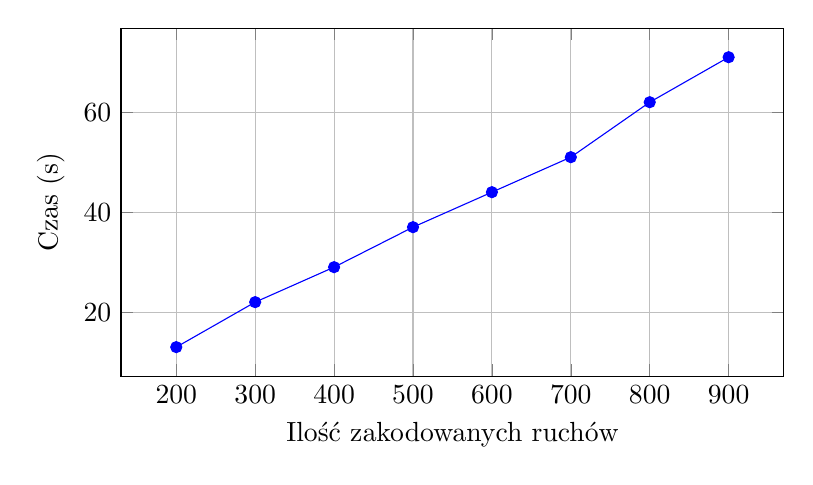
\begin{tikzpicture}
    \begin{axis}[
        xlabel={Ilość zakodowanych ruchów},
        ylabel={Czas (s)},
        grid=major,
        legend pos=north east,
        width=10cm,
        height=6cm
    ]
    \addplot[blue, mark=*] coordinates {
        (200, 13)
        (300, 22)
        (400, 29)
        (500, 37)
        (600, 44)
        (700, 51)
        (800, 62)
        (900, 71)
    };
    \end{axis}
    \end{tikzpicture}
    \caption{Czas wykonania metod concatenate po każdym zakodowaniu gry}
    \label{fig:concatenate_time}
\end{figure}


\setcounter{chapter}{1}

\chapter{Algorytm Monte Carlo Tree Search}
Zadaniem algorytmu w szachach jest znalezienie najlepszego ruchu w danej pozycji poprzez przewidywanie strategii przeciwnika. Słowo "strategia" jest kluczowe, gdyż odnosi się do planowania rozgrywki w przód, w celu realizacji zamierzeń w przyszłości, a nie tylko w obecnym stanie. Do wykonania tego zadania służą algorytmy drzewiaste analizujące różne kombinacje ruchów graczy. Takim algorytmem jest Monte Carlo Tree Search, który w połączeniu z siecią neuronową jest bardzo skutecznym algorytmem do gry w szachy.

\section{Podstawowa wersja MCTS}
Algorytm Monte Carlo Tree Search jest heurystycznym algorytmem przeszukiwania przestrzeni stanów. Jego kluczową zaletą jest iteracyjność, dzięki czemu w zależności od dostępnej mocy obliczeniowej (czasu) jest w stanie stworzyć dowolnie duże drzewo, gdzie po każdej iteracji jest gotowy zwrócić najlepszy dotychczasowy ruch. Działanie tego algorytmu opiera się na czterech etapach: selekcji, ekspansji, symulacji oraz wstecznej propagacji.

\begin{figure}[!ht]
\centering
\includegraphics[width=0.8\textwidth]{images/mcts_sections.png}
\caption{Etapy algorytmu Monte Carlo Tree Search. Źródło: GeeksforGeeks, Monte Carlo Tree Search (MCTS) in Machine Learning}
\end{figure}

\newpage

\subsection{Selekcja}
Podczas etapu selekcji algorytm wybiera najlepszą ścieżkę od korzenia drzewa do liścia poprzez wybór odpowiednich węzłów. Są one wybierane na podstawie funkcji UCT:

\begin{equation}
\operatorname{UCT}(s,a) \,=\, \widehat{Q}(s,a) \, + \, c\, \sqrt{\frac{\ln(N(s))}{N(s,a)}},\,
\quad
\widehat{Q}(s,a) \,=\, \dfrac{W(s,a)}{N(s,a)}\,
\end{equation}

\noindent gdzie:
\begin{description}
  \item[$N(s)$] - liczba odwiedzin stanu $s$
  \item[$N(s,a)$] - liczba odwiedzeń akcji $a$ w stanie $s$
  \item[$W(s,a)$] - wartość sumy nagród akcji $a$ w stanie $s$
  \item[$c$] - współczynnik eksploracji
\end{description}

\hspace{1cm}

Wzór ten składa się z sumy dwóch składników. Pierwszy z nich $\widehat{Q}(s,a)$ odpowiada za eksploatację, czyli wybór węzła, który jak dotąd osiągnął najlepszy wynik. Natomiast drugi $c\, \sqrt{\frac{\ln(n_s)}{n_{s,a}}}$ skupia się na eksploracji. Na rysunku 2.2 można zauważyć, że współczynnik ten znacznie bardziej faworyzuje mniejszą liczbę odwiedzin $n_{s,a}$. Ponadto użycie logarytmu naturalnego sprawia, że zmiana liczby odwiedzin węzła rodzica nie powoduje nagłych zmian. Współczynnik $c$ pozwala dostosować balans między eksploracją, a eksploatacją. W opisywanym algorytmie jest ustawiona standardowa wartość $c = \sqrt{2}$ = 1,41.

\begin{figure}[!t]
\centering
\begin{tikzpicture}
\begin{axis} [
    xlabel={Liczba odwiedzin węzła $n(s,a)$},
    ylabel={Wartość eksploracji},
    grid=major,
    width=10cm,
    height=6cm,
    domain=1:30,
    samples=200
]
\addplot[blue, thick] {sqrt(ln(50)/x)};
\legend{$\sqrt{\frac{\ln 50}{n(s,a)}}$}
\end{axis}
\end{tikzpicture}
\caption{Składnik eksploracji $\sqrt{\frac{\ln(N(s))}{N(s,a)}}$ dla $N(s)=50$}
\label{fig:uct-exploration}
\end{figure}

\newpage

\subsection{Ekspansja}
Etap ekspansji ma za zadanie rozbudowywać drzewo o kolejne węzły. Są one wybierane w sposób losowy spośród wszystkich możliwych akcji w danym stanie.

\subsection{Symulacja}
Etap symulacji polega na przeprowadzeniu symulacji rozgrywki od nowo dodanego węzła do końca gry w sposób losowy. W przypadku szachów oznacza to wykonywanie losowych ruchów aż do osiągnięcia stanu końcowego: mat, pat, remis.

\subsection{Wsteczna propagacja}
Ostatnim krokiem w algorytmie jest wsteczna propagacja. Ma ona na celu zaktualizowanie statystyk węzłów znajdujących się na wybranej ścieżce. W każdym z nich jest modyfikowana liczba odwiedzin oraz wartość zwrócona z symulacji.

\section{Połączenie MCTS z siecią neuronową}
Algorytm Monte Carlo Tree Search w podstawowej wersji korzysta z naiwnej metody oceniającej obecny stan gry. W grach takich jak kółko i krzyżyk, gdzie przestrzeń stanów jest bardzo ograniczona, jest to wystarczające rozwiązanie i przy odpowiedniej liczbie iteracji skuteczne. Natomiast w bardziej złożonych, jak przedstawiane szachy, taki sposób oceny staje się niewystarczający. Rozwiązaniem jest połączenie MCTS z siecią neuronową, która będzie w stanie ocenić obecny stan gry oraz przedstawić rozkład prawdopodobieństwa wszystkich następnych ruchów. Takie podejście wymaga stworzenia dwóch oddzielnych sieci, lub jednej z dwoma grupami wyjść, gdzie jedna z nich będzie siecią policy, a druga value.

W celu integracji MCTS z siecią neuronową, funkcja UCT została zastąpiona PUCT (Predictor + UCT). Takie samo podejście zostało zastosowane w AlphaZero \cite{AlphaZero}. Różnica między UCT a PUCT występuje w obliczaniu eksploracji, gdzie między innymi jest uwzględniane prawdopodobieństwo ruchu $P(s,a)$ zwracane przez sieć policy. Dodatkowo informacja z sieci value jest wstecznie propagowana w drzewie, zastępując prostą nagrodę z symulacji.
\hspace{2cm}

\begin{equation}
\operatorname{PUCT}(s,a) \,=\, \widehat{Q}(s,a) \, + \, c_{\mathrm{puct}}\, P(s,a)\, \frac{\sqrt{N(s)}}{1 + N(s,a)}\, ,
\quad
\widehat{Q}(s,a) \,=\, \dfrac{W(s,a)}{N(s,a)}\,
\end{equation}

\noindent gdzie:
\begin{description}
  \item[$\widehat{Q}$] - średnia wartość akcji $a$ w stanie $s$
  \item[$N(s)$] - liczba odwiedzin stanu $s$
  \item[$N(s,a)$] - liczba odwiedzeń akcji $a$ w stanie $s$
  \item[$P(s,a)$] - prawdopodobieństwo wyboru akcji $a$ w stanie $s$ zwracane przez sieć neuronową
  \item[$c_{puct}$] - współczynnik eksploracji
  \item[$W(s,a)$] - wartość sumy nagród akcji $a$ w stanie $s$
\end{description}

\hspace{2cm}

Dodatkowo ze względu na fakt, że szachy są grą dla dwóch graczy o przeciwnych celach, podczas wstecznej propagacji wartość zwrócona przez sieć value jest każdorazowo odwracana przy przejściu przez węzeł. Podobnie jest podczas obliczania funckji PUCT, gdzie składnik eksloatacji jest odwracany, gdyż z perspektywy węzła rodzica wartość ta musi być minimalizowana, a nie maksymalizowana. Oprócz odwracania, składnik jest normalizowany do przedziału [0,1].

Operacja odwracania oraz normalizowania składnika eksploatacji jest wykonywana według wzoru:
\begin{equation}
\widehat{Q}(s,a) \,=\,
\begin{cases}
0, & N(s,a) = 0 \\
1 - \dfrac{Q(s,a) + 1}{2}, & N(s,a) > 0
\end{cases}
\end{equation}

\section{WDL}
W algorytmie MCTS używanym w AlphaZero, wartość z value network po przepuszczeniu przez funkcję aktywacji tangensa hiperbolicznego, określa bezpośrednio wartość stanu gry. Jednakże istnieje lepszy sposób na oszacowanie wartości pozycji, który jest wykorzystywany w nowoczesnych silnikach takich jak LeelaChessZero \cite{lc0_wdl}. Zamiast przewidywać bezpośrednio wartość stanu, sieć może zwracać rozkład prawdopodobieństwa wszystkich możliwych wyników rozgrywki: wygrana, remis, przegrana. Taki sposób daje szerszy pogląd na sytuację, gdzie między innymi pozbywamy się problemu związanego z niejednoznacznością zera, które może oznaczać zarówno remis, jak i niejasną pozycję, gdzie żadna ze stron nie ma wyraźnej przewagi.

W celu zintegrowania takiego podejścia z MCTS, konieczne jest przekształcenie trzech wartości zwracanych przez sieć na jedną wartość liczbową. W tym celu jest wykonywany iloczyn skalarny wektora prawdopodobieństw:
\begin{equation}
V(s) = P_{win} \cdot 1 + P_{draw} \cdot 0 + P_{loss} \cdot (-1) = P_{win} - P_{loss}
\end{equation}

\begin{figure}[h]
\centering
\includegraphics[width=0.8\textwidth]{images/WDL.png}
\caption{Wykres rozkładu WDL podczas trwania partii szachowej. Źródło: Leela Chess Zero, Win-Draw-Loss evaluation}
\end{figure}

\newpage

\section{First play urgency}
W podstawowej wersji MCTS podczas etapu selekcji priorytet wyboru mają nieodwiedzone węzły, które są wybierane losowo. First play urgency (FPU) zmienia tę strategię poprzez zastąpienie wartości eksploatacji wartością domyślną.

Istnieje kilka wariantów strategii FPU. Ogólna zasada zakłada, że wraz ze wzrostem tej wartości nieodwiedzone węzły są bardziej faworyzowane, gdyż może ona przykrywać wartość eksploatacji węzłów już odwiedzonych.

W przedstawianym algorytmie została użyta strategia "qFPU", w której wartość domyślna jest zastępowana wartością oczekiwaną węzła rodzica. W ten sposób nieodwiedzone węzły są faworyzowane, ale nie na tyle, aby całkowicie przykryć węzły już odwiedzone. W porównaniu do strategii ze stałą wartością jest ona znacznie bardziej adaptacyjna i dynamicznie dostosowuje się do sytuacji \cite{Cazenave2021}. 

Dla przykładu, w sytuacji gdy obecna pozycja jest niekorzystna (w skutek czego FPU przyjmie niską wartość), algorytm nabierze charakteru mocno eksploatacyjnego. Będzie on unikał ryzykownych gałęzi do momentu znalezienia ruchu poprawiającego pozycję. Jeżeli taki ruch zostanie znaleziony, algorytm zacznie go wyraźnie faworyzować. Dzięki takiemu podejściu aktywnie szuka ucieczki z trudnej sytuacji, zamiast tracić czas na eksplorację potencjalnie jeszcze gorszych ruchów, jak miałoby to miejsce w przypadku stałej, wysokiej wartości FPU. 

Natomiast jeżeli FPU będzie miało wysoką dodatnią wartość, algorytm skupi się na eksploracji, aby zwiększyć szansę na znalezienie ruchu potencjalnie jeszcze lepszego niż dotychczas znaleziony.
\setcounter{chapter}{3}

\chapter{Architektura sieci neuronowej}
Architektura sieci neuronowej wykorzystywana w opisywanym rozwiązaniu jest inspirowana modelem użytym w \textit{AlphaZero}. Aczkolwiek od czasu powstania modelu od \textit{DeepMind} mineło już kilka lat, gdzie w tym czasie powstało kilka nowych technik i ulepszeń. Zostaną one przybliżone w tym rozdziale.

\section{Architektura}
Jak zostało wspomniane w poprzednim rozdziale, sieć neuronowa jest kręgosłupem algorytmu MCTS. To właśnie ona odpowiada za stworzenie dwóch rozkładów prawdopodobieństwa na podstawie dostarczanych planszy. Odpowiednio dla ruchów oraz wyniku partii. W związku z tym, podobnie jak ma to miejsce w \textit{AlphaZero}, sieć posiada jedno wejście oraz dwie grupy wyjść. Wejściem są zakodowane trzy plansze szachowe tworzące spójną sekwencję czasową. Pozwala to sieci na lepsze zrozumienie gry, gdyż widzi płynny przebieg rozgrywki, a nie jedynie pojedyńczy stan. Również zyskujemy większą różnorodność danych. W przypadku dostarczania tylko jednego stanu, jest znacznie większe prawdopodobieństwo powtarzania się takich samych danych treningowych, gdzie sieć może mieć problem z uogólnieniem wiedzy.

Dzięki dwóm grupom wyjść, sieć jest mniej obciążająca obliczeniowo niż dwie oddzielne sieci. Ponadto taka sieć we wspólnym trzonie jest zmuszona do generalizacji cech rozgrywki, co przyczynia się do lepszej regaluaryzacji modelu \cite{AlphaGoZero}. Dopiero po rozdzieleniu na dwie części, sieć specjalizuje się w swoich zadanich.

Na rysunku 3.1 przedstawiony jest diagram architektury sieci neuronowej. Zawiera on warstwy rezydualne, SE oraz dwie głowice wyjściowe. W następnej części tego rozdziału zostaną one szczegółowo omówione.


\newpage

\begin{figure}[!h]
\centering
\includegraphics[width=0.6\textwidth]{images/netArchitecture.png}
\caption{Architektura sieci neuronowej}
\end{figure}

\newpage

\section{Warstwa rezydualna}

Najważniejszym elementem przedstawianej architektury są warstwy rezydualne. Rozwiązują one oproblem z degradacją gradientu. Objawia się on przez nasyconą dokładność danych treningowych, która nie jest w stanie się poprawić. Nie jest to spowodowane przeuczeniem, lecz głębokością samej sieci. Przez co wbrew intuicji, płytszy model może osiągnąć lepsze wyniki.

W celu rozwiązania tego problemu, powstała koncepcja warstw rezydualnych. Zmieniają one sposób przepłwu informacji przez sieć. Zamiast uczyć się bezpośrednio funkcji $H(x)$, warstwa rezydualna uczy się różnicy $F(x) = H(x) - x$. Wyjściem z warstwy jest suma $F(x) + x$. W rezultacie sieć uczy się jedynie zmiany sygnału, a nie całej funkcji. Bardzo dużą zaletą tego podejścia jest stosunkowe proste stworzenie funkcji tożsamościowej poprzez wyzerowanie wag. W ten sposób autorzy w swojej pracy, pokazali że sieci rezydualne nie tworzą większego błędu niż płytsze modele \cite{ResNet}.

Na rysunku 4.2 przedstawiona jest standardowa architektura warstwy rezydualnej. Składa sie ona z 2 warstw konwolucyjnych wpieranych przez warstwy normalizacji batchowej oraz funkcje aktywacji.

\hspace{0.5cm}

\begin{figure}[!h]
\centering
\includegraphics[width=1.0\textwidth]{images/resNet.png}
\caption{Architektura warstwy rezydualnej. Kolorem niebieskim zaznaczono skip connection.}
\end{figure}

\subsection{Warstwa konwolucyjna}
Warstwa konwolucyjna jest fundamentem wykorzystywanej sieci neuronowej. To ona odpowiada za analizę oraz generalizację cech planszy szachowej. Pierwotnie została zaprojektowana do analizy obrazów, jednak równie dobrze sobie radzi z danymi przestrzennymi, takimi jak plansza szachowa. 

Nazwa pochodzi od operacji matematycznej zwanej konwolucją \footnote{W bibliotekach do uczenia maszynowego używa się podobnej funkcji zwanej cross-correlation, która działa identycznie jak konwolucja, ale nie odwraca kernela \cite{DeepLearning}.}. Polega ona na przesuwaniu kernela po wejściowej macierzy i wykonywaniu iloczynu skalarnego między filtrem, a fragmentem obrazu. Wynikiem jest mapa cech, która zawiera wyodrębnione cechy z oryginalnego obrazu. Dodatkowo, dzięki temu że kernel jest mniejszy niż obraz, to nie jest on w pełni połączony z wejściem, tak jak ma to miejsce w warstwach gęstych. Tym sposobem nie tylko ograniczamy liczbę parametrów, ale również sieć uczy się lokalnych wzorców \cite{DeepLearning}. W przypadku szachów mogą to być różne wzorce pozycyjne. 

Jak było wspomniane przy opisie przetwarzania danych, sieć konwolucyjna poprzez przesuwanie kernela, jest odporna na translacje. Oznacza to, że niezależnie od położenia figury na planszy, sieć jest w stanie rozpoznać jej cechy. Jednakże, o ile radzi sobie z translacją, to ma problem z rotacją, przez co w przetwarzaniu danych konieczne było ujednolicenie pozycji planszy do jednej orientacji \cite{DeepLearning}.

W przedstawionym modelu wykorzystywane są warstwy konwolucyjne o standardowym rozmiarze kernela $3 \times 3$ oraz stride 1 w celu zachowania rozmiaru obrazu. Podobnie jak w AlphaZero \cite{AlphaZero}, nie zostały wykorzystne warstwy poolingowe. Głównym powodem jest fakt, że o ile są w stanie bardziej ougólnić cechy, to traci się przez to informacje przestrzenne oraz małe detale obrazu \cite{DeepLearning}.

Dodatkowo należy wspomnieć, że wraz z głębokością sieci, rośnie pole recepcyjne. Oznacza to, że neurony w głebszych warstwach analizują ze sobą coraz to większe fragmenty obrazu wejściowego \cite{DeepLearning}.

\hspace{0.5cm}

\subsection{Normalizacja batchowa}
Normalizacja batchowa jest techniką adaptacyjnej reparametryzacji danych. Jej celem jest eliminacja zjawiska wewnętrznego przesunięcia kowariancji (ang. \textit{internal covariate shift}) \cite{BatchNormalization}. Objawia się ono poprzez zmieniający się rozkład wyjścia z warstw sieci neuronowej podczas adaptacji parametrów w trakcie uczenia. Innymi słowy, warstwy sieci są zależne od siebie nawzajem, przez co zmiana wag w jednej z nich wpływa na pozostałe. Prowadzi to do problemów ze stabilnością oraz doborem optymalnego współczynnika uczenia, skutkując często eksplodującymi lub zanikającymi gradientami.

Jeżeli dla przykładu rozważymy sieć neuronową bez biasu oraz z tożsamościową funkcją aktywacji, to w sytuacji, gdy wagi są większe od 1, wyjście sieci po aktualizacji parametrów zmieni się znacząco z powodu mnożenia wag (wzór 4.1). Oznacza to, że nawet mała zmiana wag w jednej warstwie może spowodować dużą zmianę na wyjściu sieci, szczególnie w głębokich modelach \cite{BatchNormalization}, nawet przy zastosowaniu małego współczynnika uczenia \cite{DeepLearning}.

\hspace{0.5cm}

\begin{equation}
\hat{y} = x \cdot (w_1 - \epsilon g_1)(w_2 - \epsilon g_2)\cdots(w_\ell - \epsilon g_\ell)
\end{equation}

\hspace{0.5cm}

W celu rozwiązania tego problemu, normalizacja batchowa normalizuje wyjście z warstwy na podstawie wyliczonej średniej oraz odchylenia standardowego całego batcha. W rezultacie rozkład danych posiada średnią równą zeru oraz jednostkowe odchylenie standardowe.

\hspace{0.5cm}

\begin{equation}
    H' = \frac{H-\mu}{\sqrt{\sigma^2 + \epsilon}}
\end{equation}

\hspace{0.5cm}

gdzie $\mu$ to średnia, $\sigma$ to odchylenie standardowe, a $\epsilon$ to mała stała zapewniająca stabilność numeryczną (zapobiega dzieleniu przez zero).

\newpage

\begin{figure}[h]
\centering
\includegraphics[width=0.4\textwidth]{images/przed_norm.png}
\hspace{0.5cm}
\includegraphics[width=0.4\textwidth]{images/po_norm.png}
\caption{Normalizacja. Dane są centrowane i skalowane, dzięki czemu zachowują swój kształt, lecz zmieniają zakres wartości.}
\end{figure}

Poniższe wzory prezentują mechanizm wstecznej propagacji błędu w opisanej wyżej prostej sieci. Ukazują one źródło problemu z niestabilnością gradientu oraz sposób, w jaki normalizacja batchowa go rozwiązuje. W równaniu 4.4 przedstawiony jest wzór na gradient w warstwie $n$ po wykonaniu różniczkowaniu wzoru 4.3. Składa się on z trzech czynników: pochodnej funkcji błędu, błędu z warstw wyższych oraz wejścia z warstwy poprzedniej ($h_{n-1}$). To właśnie ten ostatni człon jest kluczowy. We wzorze 4.5 widać, że sygnał wejściowy $h_{n-1}$ zależy od iloczynu wag warstw poprzednich. W rezultacie, w sieci bez wykonywania normalizacji, może dojść do eksplozji lub zaniku gradientu, gdy wagi są odpowiednio duże lub małe.

Zastosowanie normalizacji na $h_{n-1}$ eliminuje ten problem, niwelując zależność sygnału od skali wag. Prowadzi to do nietypowego zjawiska, w którym większe wagi skutkują mniejszymi gradientami \cite{BatchNormalization}. Dzięki temu sieć uczy się stabilniej, co pozwala na użycie większego współczynnika uczenia.

\begin{equation}
g_n=\frac{\partial L}{\partial \hat{y}} \cdot \frac{\partial \hat{y}}{\partial h_{l}} \cdot \frac{\partial h_{l-1}}{\partial h_{l-2}} \cdot ... \cdot
\frac{\partial h_{n}}{\partial w_{n}}
\end{equation}

\hspace{0.5cm}

\begin{equation}
g_{n} = \frac{\partial L}{\partial \hat{y}} \cdot \underbrace{\left( \prod_{i=n+1}^{l} W_{i} \right)}_{\text{błąd z warstw wyższych}} \cdot \underbrace{h_{n-1}}_{\text{sygnał wejściowy}}
\end{equation}

\hspace{0.5cm}

\begin{equation}
h_{n-1} = x \cdot \prod_{i=0}^{n-1} W_{i}
\end{equation}

Należy jednak zauważyć, że po znormalizowaniu wyjścia z warstwy, sieć może stracić zdolności do ekspresji. Na przykład dla funkcji ReLU uniemożliwia to całkowite wygaszenie neuronu, a dla funkcji sigmoidalnej ogranicza wykorzystanie nieliniowych obszarów funkcji nasycenia, gdzie dane głównie mogą oscylować wokół środka, gdzie ma ona postać funkcji liniowej. Aby rozwiązać ten problem, algorytm normalizacji batchowej wprowadza dwa uczone parametry: skalę $\gamma$ oraz przesunięcie $\beta$. Pozwala to sieci na zastosowanie dowolnej średniej oraz odchylenia standardowego \cite{DeepLearning}. Istotne jest to, że współczynnik $\beta$ przejmuje rolę biasu. Z tego powodu w warstwach poprzedzających normalizację batchową bias jest wyłączony. Nawet gdyby był obecny, jego wpływ zostałby zniwelowany w procesie odejmowania średniej $\mu$.

\begin{equation}
    H'' = \gamma H' + \beta
\end{equation}

\newpage

\section{Squeeze and Excitation} 
Kolejnym elementem widocznym na diagramie 4.1 są bloki \textit{Squeeze and Excitation}. Bardzo podobne rozwiązanie zostało zastosowane w LolaChessZero {\cite{lc0_nn}} Ich zadaniem jest adaptacyjna rekalibracja kanałów cech na wyjściu z warstwy konwolucyjnej. Dzięki temu niwelują one ograniczenia splotu, który analizuje jedynie lokalne wzorce, traktując zależności między kanałami w sposób niejawny \cite{SqueezeAndExcitation}. Ograniczenie to wynika przede wszystkim z użycia niewielkiego filtra, który operuje na małym fragmencie wejścia, a następnie sumuje wyniki ze wszystkich kanałów.

W celu ulepszenia warstw konwolucyjnych, blok \textit{Squeeze and Excitation} składa się z dwóch etapów: \textit{Squeeze} oraz \textit{Excitation}. Pierwszy z nich ma na celu stworzenie deskryptora globalnych cech dla każdego kanału. Osiąga się to poprzez zastosowanie globalnego uśredniania, które redukuje wymiary kanału do pojedynczej wartości.

Natomiast zadaniem \textit{Excitation} jest wychwycenie nieliniowych zależności między kanałami oraz wygenerowanie wag dla każdego z nich. Jest to realizowane za pomocą dwóch warstw gęstych rozdzielonych funkcją SiLu. Na wyjściu jest funkcja sigmoidalna z której wychodzą wartości w przedziale [0,1]. Dodatkowo, w celu ograniczenia liczby parametrów oraz poprawy generalizacji modelu, wprowadzono współczynnik redukcji \cite{SqueezeAndExcitation}. Zmniejsza on wyjście pierwszej warstwy, po czym druga warstwa przywraca pierwotną liczbę kanałów na wyjściu bloku.

\begin{figure}[h]
\centering
\includegraphics[width=0.2\textwidth]{images/squeezeArchi.png}
\caption{Blok Squeeze and Excitation}
\end{figure}

\newpage

\section{Funkcja aktywacji SiLU}

Ostatnim elementem architektury sieci jest funkcja aktywacji SiLU. Matematycznie jest ona definiowana jako iloczyn wejścia oraz funkcji sigmoidalnej.
\hspace{0.5cm}

\begin{equation}
    f(x) = x \cdot \sigma(x) = \frac{x}{1+e^{-x}}
\end{equation}

\hspace{0.5cm}

Dla dużych wartości dodatnich funkcja zachowuje się niemal identycznie jak ReLU, natomiast dla wartości ujemnych dąży do zera \cite{SiLu}. Jednakże, nie jest ona funkcją monotonicznie rosnącą. W punkcie $x \approx -1.28$ posiada minimum.

W tym punkcie pochodna funkcji przyjmuje wartość zerową. W rezultacie dla wartości mniejszych niż $-1.28$, funkcja wykazuje charakter samoregulujący. W tym obszarze pochodna jest ujemna, co powoduje, że podczas wstecznej propagacji błędu odwracany jest znak gradientu. Skutkiem tego jest hamowanie wzrostu wag o dużej wartości bezwzględnej. Taki mechanizm pozwala zapobiec wyłączeniu się neuronu. Należy jednak zaznaczyć, że obszar ten jest ograniczony, więc przy wystąpieniu odpowiednio dużego błędu, wprowadzenie neuronu w stan trwałej saturacji jest nadal możliwe, jak w przypadku funkcj ReLu.


\begin{figure}[h]
\centering
\includegraphics[width=1\textwidth]{images/SiLu.png}
\caption{Po lewej porównanie SiLu oraz ReLu. Po prawej pochodna SiLu (dSiLu) oraz funkcja sigmoidalna. Źródło: \cite{SiLu}}
\end{figure}
% W ATCH THE U NOBSERVED : A S IMPLE A PPROACH TO PARALLELIZING MONTE CARLO TREE SEARCH
\setcounter{chapter}{3}

\chapter{Zrównoleglenie MCTS}
Celem zrównoleglenia MCTS jest przyśpieszenie wykonywania algorytmu poprzez lepsze wykorzystanie dostępnych zasobów sprzętowych przy jednoczesnym zachowaniu jakości podejmowanych decyzji. W tym rozdziale zostanie przedstawiony i rozwiązany problem z perspektywy CPU oraz GPU.

\hspace{3cm}

\section{Metoda batchowania danych}
Frameworki do pracy z sieciami neuronowymi, takie jak wykorzystywany PyTorch, są zoptymalizowane do pracy na partiach danych. Do teraz drzewo MCTS wykonywało się w pełni sekwencyjnie, czego skutkiem było przetwarzanie tylko jednej próbki danych przez sieć neuronową.

Ulepszona koncepcja polega na dodawaniu odpowiedniej liczby liści do bufora, tak aby można było je przetworzyć w jednej partii przez sieć neuronową. Po otrzymaniu wyników z sieci, drzewo jest aktualizowane poprzez wsteczną propagację. 

Głównym problemem jest brak aktualizacji statystyk drzewa w trakcie dodawania liści do bufora. Powoduje to, że podczas etapu selekcji algorytm PUCT nie ma aktualnych informacji o stanie drzewa przez co wybierana jest ta sama ścieżka. 

Można spróbować naiwnie rozwiązać ten problem poprzez blokowanie liści dodanych do bufora, wymuszając tym samym wybór innego liścia, aczkolwiek nie jest to optymalne rozwiązanie. Mimo takiego zabiegu wybierane są różne liście, jednakże posiadające tego samego rodzica, co można zaobserwować na rysunku 4.1. Taka metoda w praktyce jest szybsza, aczkolwiek znacznie mniej efektywana niż wersja sekwencyjna.

\newpage

\begin{figure}[h]
\centering
\includegraphics[width=0.8\textwidth]{images/mcts-naive-batch.png}
\caption{Naiwna metoda batchowania danych. Czerwone strzałki reprezentują wybraną najlepszą ścieżkę. Liść oznaczony numerem 6 został dodany do bufora i jest zablokowany. Na fioletowo została oznaczona ścieżka prowadząca do kolejnego liścia, który zostanie dodany do bufora.}
\end{figure}

\section{Fundament idealnego algorytmu równoległego}

W artykule "On effective parallelization of Monte Carlo Tree Search" \cite{EffectiveParallelMCTS} autorzy definiują warunki konieczne dla statystyk węzłów, które muszą zostać spełnione aby równoległe drzewo było nie tyle co szybsze, ale również tak samo skuteczne jak sekwencyjne:

\begin{equation}
\begin{aligned}
\overline{N}(s,a) &\ge N(s,a) + O(s,a) \\
\overline{G}(s,a) &:= \lvert \mathbb{E}[\overline{Q}(s,a)] - \mathbb{E}[Q_{m}^{\mathbb{A}_{\text{seq}}}(s,a)] \rvert = 0 \quad (m=N(s,a)+O(s,a))
\end{aligned}
\end{equation}

\noindent gdzie:
\begin{description}
  \item[$\overline{N}(s,a)$] - zmodyfikowana liczba odwiedzin akcji $a$ w stanie $s$
  \item[$N(s,a)$] - liczba odwiedzin akcji $a$ w stanie $s$
  \item[$O(s,a)$] - liczba liści w których trwają obliczenia dla akcji $a$ w stanie $s$
  \item[$G(s,a)$] - (ang. Gap) błąd estymacji wartości akcji $a$ w stanie $s$
  \item[$\overline{Q}(s,a)$] - zmodyfikowana wartość akcji $a$ w stanie $s$ w algorytmie równoległym
  \item[$Q_{m}^{\mathbb{A}_{\text{seq}}}(s,a)$] - wartość akcji $a$ w stanie $s$ w algorytmie sekwencyjnym po $m$ odwiedzinach
\end{description}

\vspace{0.5cm}

Powyższe warunki konieczne pokazują, że idealny algorytm równoległy musi w trakcie oczekiwania na wynik obliczeń, modyfikować tymczasowo statystyki węzłów. Powinny one być idealnie oszacowane, tak aby drzewo w każdej chwili czasowej dysponowało aktualnymi informacjami o swoim stanie. W przeciwnym razie, algorytm opierający swoje działanie na nieaktualnych wartościach dokonywałby nieoptymalnych wyborów węzłów, co można było zaobserwować na rysunku 4.1.

W praktyce spełnienie pierwszego warunku jest stosunkowo proste i zostało to rozwiązane przez implementacje WU-UCT, natomiast drugi warunek jest bardzo trudny do zrealizowania, gdyż wymaga przewidzenia wartości akcji.

\section{WU-UCT - Watch the Unobserved}
Metoda WU-UCT ma na celu spełnienie pierwszego z warunków koniecznych przedstawionych w równaniu (4.1). Wprowadza ona dodatkową zmienną $O(s,a)$, która przechowuje informację o liczbie liści, dla których trwają obecnie obliczenia w akcji $a$ w stanie $s$. W momencie wyboru liścia, wartość tej zmiennej jest inkrementowana dla każdego węzła na wybranej ścieżce. Po otrzymaniu wyniku, jest ona dekrementowana w trakcie wstecznej propagacji.

Zmienna $O(s,a)$ jest wykorzystywana w zmodyfikowanym wzorze PUCT do uzupełnienia informacji o liczbie odwiedzin węzła. W efekcie algorytm dynamicznie koryguje wartość eksploracji w zależności od liczby trwających obliczeń węzłów potomnych. Wyższa wartość $O(s,a)$ skutkuje mniejszą wartością eksploracji. Pozwala to na unikanie podążania za ścieżkami, w których trwają już obliczenia, skupiając się na eksploracji innych części drzewa.

Mechanizm blokowania przedstawiony w podrozdziale 4.1, pełni teraz tylko rolę zabezpieczenia. Zapewnia on, że do bufora nie zostanie dodany ten sam liść. W najgorszym przypadku zostanie dodany najlepszy liść tego samego rodzica, który nie znajduje się w buforze.

\vspace{1cm}

\begin{equation}
\operatorname{WU-UCT}(s,a) \,=\, \widehat{Q}(s,a) \, + \, c_{\mathrm{puct}}\, P(s,a)\, \frac{\sqrt{(\sum_{b} N(s,b)) + O_s}}{(1 + N(s,a)) + O_s}\, ,
\end{equation}
\noindent gdzie:
\begin{description}
  \item[$\widehat{Q}$] - średnia wartość akcji $a$ w stanie $s$
  \item[$N(s)$] - liczba odwiedzin stanu $s$
  \item[$N(s,a)$] - liczba odwiedzeń akcji $a$ w stanie $s$
  \item[$\sum_{b} N(s,b)$] - suma odwiedzin wszystkich akcji w stanie $s$
  \item[$P(s,a)$] - prawdopodobieństwo wyboru akcji $a$ w stanie $s$ zwracane przez sieć neuronową
  \item[$c_{puct}$] - współczynnik eksploracji
  \item[$O_s$] - suma trwających obliczeń węzłów potomnych stanu $s$
\end{description}

\begin{figure}[h]
\centering
\includegraphics[width=0.8\textwidth]{images/WU-UCT.png}
\caption{WU-UCT. Czerwona strzałka przedstawia najlepszą ścieżkę, natomiast fioletowa przedstawia ścieżkę do kolejnego liścia dodawanego do bufora}
\end{figure}

\newpage

Na poniższym listingu można zauważyć bardzo dużą różnicę między naiwnym blokowaniem wybranych liści, a wykorzystaniem metody WU-UCT. Dzięki spełnieniu pierwszego warunku koniecznego, algorytm WU-UCT skuteczniej eksploruje drzewo, wybierając liście z różnych części drzewa, a nie tylko z tej samej gałęzi.

\begin{lstlisting}[
    language=Python,
    caption=Adresy rodziców 8 liści znajdujących się w buforze,
    inputencoding=utf8,
    basicstyle=\ttfamily\footnotesize,
    backgroundcolor=\color{gray!10},
    frame=single,
    showspaces=false,
    showstringspaces=false,
    numbers=none
]
Blokowanie:
0x705d41c78440
0x705d41c78440
0x705d41c78440
0x705d41c78440
0x705d41c78440
0x705d41c78440
0x705d41c78440
0x705d41c78440

WU-UCT:
0x7a5e5d1e1be0
0x7a5e5d1e38f0
0x7a5e5d1f1640
0x7a5e5d1f3350
0x7a5e5d0010a0
0x7a5e5d002db0
0x7a5e5d00cb00
0x7a5e5d00e810
\end{lstlisting}

\newpage

\section{Wady batchowania danych}
Przedstawione podejście batchowania danych rozwiązuje problem nieoptymalnego wykorzystania GPU. Jednakże po rozwiązaniu problemu narodziły się kolejne.

Algorytm WU-UCT spełnia tylko pierwszy z warunków koniecznych przedstawionych w równaniu (4.1). Drugi warunek mówiący o idealnym oszacowaniu wartości akcji nadal nie jest spełniony. W praktyce oznacza to, że drzewo MCTS nie posiada idealnych informacji o swoim stanie, przez co wraz ze wzrostem rozmiaru bufora zwiększa się bias algorytmu.

Kolejnym występującym problemem jest sam język Python. Jest on językiem interpretowanym, przez co niespodziewanym wąskim gardłem stały się najprostsze operacje utrzymujące drzewo. Szczególnie jest to widoczne przy etapie ekspansji, gdzie czas wykonania wynosi $O(n * m)$, gdzie $n$ to wielkość bufora, a $m$ to liczba możliwych ruchów z danego stanu (średnio ok 45). Taka pętla jest znacznie wolniejsza niż sama sieć neuronowa, przez co zwiększanie rozmiaru bufora nie przekłada się na duży wzrost szybkości wykonania.

W efekcie powyższych problemów, zwiększanie rozmiaru bufora nie tylko nie przekłada się na widoczną poprawę czasu wykonania, ale również pogarsza się jakość podejmowanych decyzji.

\begin{figure}[!h]
\centering
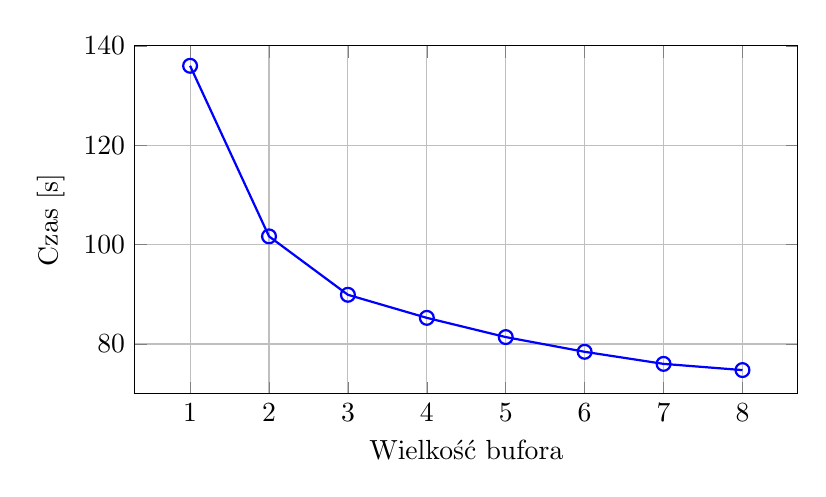
\begin{tikzpicture}
  \begin{axis}[
      width=10cm,
      height=6cm,
      grid=both,
      xlabel={Wielkość bufora},
      ylabel={Czas [s]},
      xtick={1,2,3,4,5,6,7,8},
      ymin=70,
      ymax=140,
      ymajorgrids=true,
      xmajorgrids=true,
      legend style={at={(0.02,0.98)},anchor=north west,font=\small},
      mark size=2.5pt
  ]
    \addplot+[blue, thick, mark=o] coordinates {
      (1,135.98)
      (2,101.66)
      (3,89.9)
      (4,85.26)
      (5,81.39)
      (6,78.43)
      (7,76.0)
      (8,74.75)
    };
  \end{axis}
\end{tikzpicture}
\caption{Wpływ wielkości bufora na czas wykonania 6000 iteracji}
\label{fig:metric-iteracje}
\end{figure}

Testy wydajnościowe przedstawione na wykresie zostały przeprowadzone na procesorze i7-11800H oraz GPU RTX 3060. Na wykresie 4.3 można zaobserwować, że wraz ze wzrostem wielkości bufora, różnica czasu wykonania maleje. 

Jako optymalną wartość rozmiaru bufora wybrano 2, gdyż daje ona bardzo duży zysk czasowy, a jednocześnie brak spełenia drugiego warunku koniecznego nie ma dużego wypływu na jakość podejmowanych decyzji. Na wykresie 4.4 można zauważyć, że używając tego samogo czasu na oblieczenie ruchu, algorytm z buforem o rozmiarze 2 osiąga przewagę nad sekwencyjną wersją.
\begin{figure}[h]
\centering
\includegraphics[width=0.55\textwidth]{images/buffor-comp.png}
\caption{Rozgrywka między sekwencyjnym MCTS a MCTS z buforem o rozmiarze 2 przy tym samym czasie wykonania. Rozgrywka została oceniona przez silnik Stockfish.}
\end{figure}


\newpage

\section{Wieloprocesowy MCTS}
Do tej pory opisywane metody skupiały się na większym wykorzystaniu GPU. Jednakże dużym ograniczeniem stanowią operacje na drzewie wykonywane przez CPU. Dzisiejsze procesory posiadają stosunkowo dużą liczbę rdzeni, które można wykorzystać do przyśpieszenia obliczeń. 

Do zrównoleglenia algorytmu zostały użyte wszystkie omówione wcześniej techniki, takie jak batchowanie danych z buforem o rozmiarze 2 oraz WU-UCT. Działanie samej równoległości opiera się na metodzie tree parallelization, gdzie jedno drzewo jest współdzielone między wszystkimi workerami. 

\subsection{Struktura drzewa}
Język Python jest językiem jednowątkowym przez co koniecznym było użycie wieloprocesowości. Głównym problemem w takim podejściu jest brak współdzielonej pamięci programu między procesami. Z tego powodu konieczne było wydzielenie fragmentu pamięci dynamicznej do przechowywania współdzielonej struktury drzewa. Z poziomu Pythona ma ona postać zwykłych bajtów, przez co możliwe są tylko dwa rozwiązania przechowywania obiektowej struktury: spłaszczenie, lub użycie serializacji wraz z deserializacją. Z oczywistych względów wydajnościowych jak i prostoty implementacji została wybrana pierwsza metoda.

Ze względu na fakt, że używając współdzielonaj pamięci jest tylko dostęp do bloku bajtów, spłaszczona struktura musi być przechowywana w tablicy. Ogólne działanie drzewa jest oparte na podobnej zasadzie co wersja obiektowa. Z taką różnicą, że zamiast operować na referencjach, operujemy na indeksach tablicy. Każdy węzeł zawiera informacje o id rodzicu oraz dzieci. Statystyki drzewa są przechowywane identycznie jak w wersji obiektowej. Różnica pojawia się tylko przy stanie gry, czyli planszy. Zamiast serializować i deserializować obiekt BoardPlus, plansza jest przechowywana w znacznie bardziej kompaktowej formie, jako tablica charów oraz zmiennej bool. Opisują one kolejno stan planszy w formacie FEN oraz perspektywę rozgrywki. Format FEN był opisywany w pierwszym rozdziale.

Każda zmienna została dobrana pod kątem minimalizacji zużycia pamięci. Przykładowo liczba odwiedzin jest przechowywana jako 16 bitowa liczba całkowita bez znaku, gdyż w praktyce nie zdarza się aby liczba odwiedzin przekroczyła 65535 oraz była ujemna. Dodatkowo ze względu na użycie tablic, wszystkie ich rozmiary są ustalane przed rezerwacją pamięci. Rozmiar drzewa jest obliczany na podstawie wzoru 4.3, gdzie brana jest pod uwagę maksymalna liczba dzieci na węzeł oraz liczba symulacji. Maksymalna liczba dzieci jest stała i wynosi 100, co jest wartością bardzo bezpieczną, gdyż średnia liczba możliwych ruchów w szachach wynosi około 45.

\vspace{0.5cm}

\begin{equation}
\operatorname{treeSize} \,=\, \operatorname{maxChildrenPerNode} \times \operatorname{simNumber} + 1
\end{equation}

\begin{lstlisting}[
    language=Python,
    caption=Struktura tablicy przechowującej drzewo MCTS w pamięci współdzielonej,
    inputencoding=utf8,
    basicstyle=\ttfamily\footnotesize,
    backgroundcolor=\color{gray!10},
    frame=single,
    showspaces=false,
    showstringspaces=false,
    numbers=none
]
tree_dtype = np.dtype([
    # -1 for root
    ('parent_id', np.int32),
    # avg max children per node is ~(30-55)
    ('children', np.uint32, MAX_CHILDREN_PER_NODE), 
    ('children_count', np.uint8),
    ('fen', 'S100'),
    ('changed_perspective', np.bool_),
    ('move_id', np.int16), # -1 for root
    ('total_visit', np.uint16),
    ('total_reward', np.float32),
    ('prior', np.float32),
    ('unobserved_samples', np.uint32),
    ('is_locked', np.bool_),
    # result for terminated states. 2 for not terminated
    ('result', np.int8)
])
\end{lstlisting}

\vspace{0.5cm}

Powyższa struktura uwzględnia również zmienną result przechowującą wynik gry dla zakończonych stanów. Wartość ta jest dodawana w momencie ekspancji. Pozwala to uniknąć niepotrzebnej kolejnej zamiany fen na obiekt klasy BoardPlus bezpośrednio po selekcji.

\vspace{2cm}

\begin{figure}[h]
\centering
\includegraphics[width=1\textwidth]{images/tree_structure.png}
\caption{Struktura drzewa w pamięci współdzielonej}
\end{figure}

\newpage

\subsection{Działanie wieloprocesowego MCTS}
Ostatnim wyzwaniem było zaprojektowanie procesów wykonawczych wraz z ich synchronizacją, gdzie każdy z nich ma za zadnie wykonanie takiej samej liczby symulacji. Trzeba wziąć pod uwagę fakt, że wszystkie operacje będą odbywały się na jednym drzewie. Szczególnie jest to problematyczne w początkowej fazie, gdzie przez dostępność małego zbioru liści, może dojść do sytuacji gdzie wiele procesów będzie podążało tą samą ścieżką osiągając ten sam liść.

Bardzo dobrze ilustruje to przypadek widoczny na rysunku 4.6, gdzie algorytm po inicjalizacji zaczyna wykonywać pierwszą selekcję zaczynając od korzenia. Naturalnie jest tylko jeden korzeń w drzwie, więc trzeba wówczas zapewnić że tylko jeden proces będzie mógł go rozwinąć, a pozostałe będą musiały czekać. Obsługa takiego przypadku jest zaprezentowana na rysunku 4.7, gdzie algorytm od razu sprawdza czy są dostępne liście. Jeżeli nie, to czeka, albo przetwarza swój bufor niezależnie od rozmiaru. Wywołanie przetwarzania bufora w takim przypadku ma na celu uniknięcie sytuacji, gdzie procesy same się blokują czekając na odblokowanie liści w buforach.

\begin{figure}[h]
\centering
\includegraphics[width=0.6\textwidth]{images/waiting-proc.png}
\caption{Procesy oczekujące na dostępne liście}
\end{figure}


Następnym bardzo ważnym aspektem w równoległości jest integralność danych. Zapewniona jest ona przez użycie dwóch blokad. Oznaczone odpowiednio jasnobrązowym oraz zielonym kolorem na rysunku 4.7 i 4.8. Widoczny duży jasnobrązowy blok odpowiada za zapewnienie atomowości operacji wyboru liścia. Dzięki temu tylko jeden proces może wykonać kolejno: wybór liścia, aktualizacje tymczasowej statystyki oraz zablokowanie. Unikamy w ten sposób sytuacji, gdzie dwa procesy przetwarzają ten sam liść.
\begin{figure}[h]
\centering
\includegraphics[width=1\textwidth]{images/multiproc-mcts.png}
\caption{Schemat procesu w wieloprocesowym MCTS}
\end{figure}

\newpage

Na rysunku 4.7 jest przedstawiona również druga blokada. Odpowiada ona za integralność zmiennej przechowującej ostatni zapisany indeks w tablicy drzewa. Jest to istotne podczas ekspansji, gdzie nowy węzeł jest tworzony na indeksie wskazywanym przez tę zmienną.
\begin{figure}[h]
\centering
\includegraphics[width=1\textwidth]{images/buffor-schematic.png}
\caption{Schemat przetwarzania bufora}
\end{figure}

\section*{Ewaluacja MCTS}
Najbardziej obiektywnym sposobem oceny działania całego algorytmu szachowego jest porównanie go z innym. Wybrany został Stockfish ze względu na jego popularność oraz wsparcie biblioteki \textit{chess} ułatwiającej integrację.

Porównanie polega na rozegraniu podanej liczby partii pomiędzy dwoma silnikami. Białe figury są reprezentowane przez Stockfish, a czarne przez opisywany model. Główną miarą oceny jest przeżywalność, czyli liczba ruchów w danej partii. Dodatkowo w celu uzyskania bardziej szczegółowych danych, stockfish w każdej rundzie podaje ocenę pozycji dla czarnych figur. Mieści się ona w przedziale od -1000 do 1000, gdzie skrajne wartości oznaczają mat.
W pliku konfiguracyjnym użytkownik za pomocą wartości \textit{stockfish\_gen\_moves} może ustawić ilość generowanych ruchów przez Stockfish w danej turze. Spośród nich jest losowany ostateczny ruch. Taki mechanizm pozwala na znaczne obniżenie poziomu trudności silnika. Było to szczególnie bardzo istotne w początkowej fazie rozwoju modelu, gdzie jego skuteczność była niska. Obecnie ze względu na dobrą jakość implementowanego algorytmu, wartość ta jest ustawiona na 1, co oznacza że Stockfish nie jest osłabiany.

Na wykresach porównawczych jest również uwzględniony wynik losowego modelu, który w każdej turze wybiera losowy (legalny) ruch. Pełni on rolę poziomu odniesienia.

\begin{figure}[h]
\centering
\includegraphics[width=0.6\textwidth]{images/stockfish.png}
\caption{Wykres przeżywalności modelu względem Stockfish}
\end{figure}

\setcounter{chapter}{4}
\chapter[Architektura aplikacji serwerowej {[\textit{Michał Lichtarski}]}]{Architektura aplikacji serwerowej}

W tej części zostanie przybliżona architekrura aplikacji serwerowej na której opiera się cała omawiana praca.

\section{Komunikacja GUI z silnikiem szachowym}
Do komunikacji z silnikiem szachowym została stworzona klasa \textit{Communication}. Działa ona w oparciu o \textit{sockety}, gdzie każdy klient jest obłusgiwany w osobnym wątku. Ze względu na ograniczenia wydajnościowe, niezależnie od ilości klientów działa tylko jedna instancja silnika szachowego. W momencie otrzymania zapytania od klientów, wiadomości są kolejkowane i obsługiwane w kolejności ich nadejścia.

Wiadomości są w postaci \textit{JSON} i zawierają następujące 2 pola: \textit{command} oraz \textit{boards}. Pole \textit{command} zawiera komendę do wykonania. W obecnej wersji jest tylko jedna komenda \textit{get\_move}, która przekazuje do silnika szachowego aktualne stany plansz i zwraca odpowiedź z najlepszym ruchem. Pole \textit{boards} zawiera listę stanów planszy w formacie \textit{FEN}. Silnik podejmuje decyzję o ruchu na podstawie do 3 stanów.

\section{Interfejs aplikacji serwerowej}
Aplikacja serwerowa obługiwana jest poprzez prosty interfejs konsolowy, pozwalający na wywoływanie funkcji. Po wpisaniu komendy \textit{help} wyświetlana jest lista dostępnych komend wraz z ich krótkim opisem. Dodatkowo wyświetlone są parametry jakie obsługują. Kwadratowe nawiasy oznaczają parametry opcjonalne. W celu lepszej automatyzacji serwera, w pliku konfiguracyjnym pod nazwą \textit{startCommands} można wpisać listę komend wraz z argumentami, które zostaną automatycznie wywołane po starcie aplikacji.

\newpage

\begin{figure}[h]
\centering
\includegraphics[width=1\textwidth]{images/app_interfejs.png}
\caption{Interfejs aplikacji serwerowej}
\end{figure}

\section{Testowe środowisko klienckie}
Do testowania aplikacji serwerowej została stworzona prosta graficzna aplikacja kliencka, która umożliwia grę w szachy. Została stworzona w języku Python z wykorzystaniem biblioteki PyGame. Działanie opiera się na zamianie obiektu board z biblioteki chess na plansze szachową z figurami, gdzie każda z nich jest w postaci zdjęcia z usuniętym tłem. Umożliwia również wykonywanie ruchów białymi figurami przez użytkownika. Interfejs graficzny dopuszcza i pokazuje tylko poprawne ruchy. W momencie gdy jest tura przeciwnika, wywoływany jest listener zwracający obiekt move. Taka struktura pozawala na bardzo łatwą implementację dowolnego algorytmu. 

W tym przypadku w listenerze jest wysyłane zapytanie do aplikacji serwerowej z aktualnymi stanami planszy. Po otrzymaniu odpowiedzi ruch jest wykonywany na planszy.

\begin{figure}[h]
\centering
\includegraphics[width=0.4\textwidth]{images/gui_czyste.png}
\hspace{1cm}
\includegraphics[width=0.4\textwidth]{images/gui_ruch.png}
\caption{intefejs graficzny}
\end{figure}

\newpage

\lstset{style=codeListingStyle}
\begin{lstlisting}[
    language=Python, 
    caption=Przykładowe użycie gui,
    inputencoding=utf8
]
# obiekt board na ktorym dziala cala gra
board = BoardPlus()
game = ChessGUI(board)
communication = Communication("localhost", 12345)

def algorithm():
    communication.send({
        "command": "get_move",
        "boards": game.get_last_states(3)
    })

    start = time.time()
    while not communication.is_message_available():
        # timeout
        if time.time() - start > 150:
            raise TimeoutError("No response from the chess engine.")
        sleep(1)

    message = communication.get_message()
    move = chess.Move.from_uci(message["move"])

    return move

game.add_computer_algorithm_listener(algorithm)
game.run()
\end{lstlisting}
\section*{Wnioski}
Na podstawie przeprowadzonych eksperymentów można stwierdzić jeden główny problem opisywanego algorytmu. Jest nim niska jakość głowicy value. Jest ona przede wszystkim spowodowana słabą jakością danych treningowyc, które są generowane na podstawie końcowego wyniku partii. Oznacza to, że stany plansz nie są indywidualnie etykietowane na podstawie ich faktycznej wartości. Problem ten jest szczególnie widoczny w początkowej fazie rozgrywki, gdzie przewidzenie wyniku na podstawie samej pozycji jest praktycznie niemożliwe.
Rozwiązaniem może być zastosowanie innego silnika szachowego do tworzenia etykiet. Nadawane by były one indywidualnie dla każdego stanu, niezależnie od końcowego wyniku. Aczkolwiek celem niniejszej pracy było stworzenie od podstaw całego algorytmu, niezależnego od istniejących rozwiązań, dlatego też nie zdecydowano się na takie podejście.

\newgeometry{top=2cm, bottom=2cm, left=2.5cm, right=2.5cm}

\bibliographystyle{plain}
\bibliography{bibliography}
\end{document}